%%%%%%%%%%%%%%%%%%%%%%%%%%%%%%%%%%%%%%%%%%%%%%%%%%%%%%%%%%%%%%%%%%%%%%%%
%                                                                      %
%     File: Thesis_Conclusions.tex                                     %
%     Tex Master: Thesis.tex                                           %
%                                                                      %
%     Author: Andre C. Marta                                           %
%     Last modified :  2 Jul 2015                                      %
%                                                                      %
%%%%%%%%%%%%%%%%%%%%%%%%%%%%%%%%%%%%%%%%%%%%%%%%%%%%%%%%%%%%%%%%%%%%%%%%

\chapter{Conclusions}
\label{chapter:conclusions}
The simplistic approach of the RISC-V ISA paired with the use of RTOS enables developers of embedded systems to build optimized systems for their specific application. However, with an increase in the volume and processing requirement of data, further improvements must be done to the embedded systems that process that data. One improvement is the incorporation of hardware accelerators. 

In this initial work, an overview of the SoC and RTOS mechanism necessary is performed. From the vast variety of existing SoC, the SweRVolf is chosen as a base to build the full system. SweRVolf was chosen due to its complete documentation, community support, and support for popular RTOS. The RTOS chosen for this system is Zephyr since its modularity and vast documentation allow the creation of a system that is optimized for this thesis application.

The preliminary work described in Chapter \ref{chapter:PreliminaryWork} presents the necessary tools to build a complete system. Utilizing already established hardware to study the RTOS basic mechanisms allowed for a further understanding of such mechanisms without the interference of possible hardware debugging. Designing a basic SoC similar to the one chosen provided knowledge on how to later add the hardware accelerator to the SoC. Finally, the use of simulation tools to build a Zephyr application targeting the designed SoC provided a basic understanding of the necessary procedures to build the final system.

The integration of an RTOS into a RISC-V based hardware accelerator requires an evaluation and analysis of performance metrics. These metrics should help to study the efficiency and resource utilization of the system. Some of the key performance metrics are: ROM and RAM utilized, FPGA area utilized, context switching delay, interrupt latency, message passing delay, and overall speedup of the application.


% ----------------------------------------------------------------------
% \section{Achievements}
% \label{section:achievements}



% ----------------------------------------------------------------------
\section{Work Plan}
\label{section:future}
Following the work already done, the next step will be to build the full SoC with the hardware accelerator. With a full SoC, the second step will be to implement the two solutions provided in Chapter \ref{chapter:PreliminaryWork}. Solution one is for every task to communicate with the accelerator separately, reducing the communication time but increasing the complexity of the tasks. Solution two is to have a central task that manages the accesses to the accelerator, adding one step to the communication process, but reducing the complexity of the tasks. After that, the study of new and improved solutions will be done. The last step is the evaluation of the developed solutions. The timeline of the work schedule can be seen in Figure \ref{fig:workplan}.

\begin{figure}[H]
    \centering
    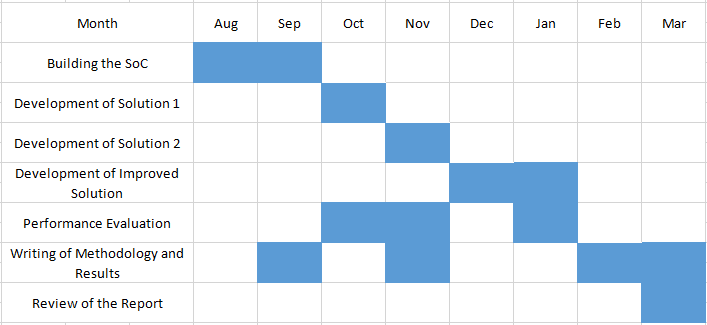
\includegraphics[scale=0.7]{Figures/workplan.png}
    \caption{Work Plan}
    \label{fig:workplan}
\end{figure}
